% !TEX TS-program = pdflatex
% !TEX encoding = UTF-8 Unicode

% This is a simple template for a LaTeX document using the "article" class.
% See "book", "report", "letter" for other types of document.

\documentclass[11pt]{article} % use larger type; default would be 10pt

\usepackage[utf8]{inputenc} % set input encoding (not needed with XeLaTeX)

%%% Examples of Article customizations
% These packages are optional, depending whether you want the features they provide.
% See the LaTeX Companion or other references for full information.

%%% PAGE DIMENSIONS
\usepackage{geometry} % to change the page dimensions
\geometry{a4paper} % or letterpaper (US) or a5paper or....
% \geometry{margin=2in} % for example, change the margins to 2 inches all round
% \geometry{landscape} % set up the page for landscape
%   read geometry.pdf for detailed page layout information

\usepackage{graphicx} % support the \includegraphics command and options

% \usepackage[parfill]{parskip} % Activate to begin paragraphs with an empty line rather than an indent

%%% PACKAGES
\usepackage{booktabs} % for much better looking tables
\usepackage{array} % for better arrays (eg matrices) in maths
\usepackage{paralist} % very flexible & customisable lists (eg. enumerate/itemize, etc.)
\usepackage{verbatim} % adds environment for commenting out blocks of text & for better verbatim
\usepackage{subfig} % make it possible to include more than one captioned figure/table in a single float
% These packages are all incorporated in the memoir class to one degree or another...
\usepackage[italian]{babel}

%%% HEADERS & FOOTERS
\usepackage{fancyhdr} % This should be set AFTER setting up the page geometry
\pagestyle{fancy} % options: empty , plain , fancy
\renewcommand{\headrulewidth}{0pt} % customise the layout...
\lhead{}\chead{}\rhead{}
\lfoot{}\cfoot{\thepage}\rfoot{}

%%% SECTION TITLE APPEARANCE
\usepackage{sectsty}
\allsectionsfont{\sffamily\mdseries\upshape} % (See the fntguide.pdf for font help)
% (This matches ConTeXt defaults)

%%% ToC (table of contents) APPEARANCE
\usepackage[nottoc,notlof,notlot]{tocbibind} % Put the bibliography in the ToC
\usepackage[titles,subfigure]{tocloft} % Alter the style of the Table of Contents
\renewcommand{\cftsecfont}{\rmfamily\mdseries\upshape}
\renewcommand{\cftsecpagefont}{\rmfamily\mdseries\upshape} % No bold!

%%% END Article customizations

%%% The "real" document content comes below...

\title{Applicazione di Hardware Metamorfico per approccio esplorativo di progettazione di Sistemi Embedded}
\author{Enrico Giordano}
\date{} % Activate to display a given date or no date (if empty),
         % otherwise the current date is printed 

\begin{document}
\maketitle

\section{Introduzione}

Il flusso di progettazione standard di un sistema embedded si divide in tre step: analisi, progettazione e sintesi; questo flusso mira ad avere un sistema specifico per una situazione particolare e alla sintesi finale di tale sistema il meno generale possibile, in modo da renderlo massimamente performante per quel particolare ambiente. Il flusso standard prevede un particolare sforzo durante l'analisi, in particolare l'analisi ambientale, in quanto è necessario capire esattamente il contesto in cui verrà calato il sistema.

Con questa tesi, si vuole proporre un approccio alternativo il cui mezzo è l'utilizzo di hardware metamorfico e quindi di una particolare tecnica di progettazione basata sulla ``configurabilità parziale'' della tecnologia delle FPGA. Usando questo mezzo, si vuole progettare un sistema più generico possibile e, calato in un contesto particolare, sarà in grado di modificarsi in base alle esigenze del luogo, per poi generare un sistema embedded autoformato e specifico per l'ambiente. Basandosi sul concetto di ``evoluzione'', secondo cui un oggetto si modifica in base all'ambiente, si otterrà per ogni ambiente un particolare sistema embedded. Estraendo poi dalla FPGA il codice ottenuto durante l'evoluzione, si potrà ottenere il codice finale e specifico per una ASIC, che quindi non verrà più modificato.

Si presenteranno quindi, a livello descrittivo, le diverse tecniche di configurabilità parziale, introducendo poi un modello di progettazione che mira ad un approccio standardizzato per i futuri sviluppi di questa idea, per poi provare il tutto su un caso di studio reale.

\section{Il concetto di Hardware Metamorfico}

Il concetto di ``Hardware Metamorfico'' nasce nei primi anni del 1990, per poi perdere parzialmente interesse in quanto veniva presentato come idea, non come tecnologia pratica. Con questo concetto si intende un tipo di Hardware capace di cambiare il proprio comportamento (``evolvere'') utilizzando un ``metodo'' di riconfigurazione: i termini ``evolvere'' e ``metodo'' non sono mai stati definiti in maniera standard, il paper che cerca di porre chiarezza su tutto questo ambito \cite{MS1} focalizza l'attenzione sulle diverse sfaccettature del termine ``evoluzione'', parlando di evoluzione ``intrinseca'' , ``estrinseca'' e ``mixata'', rimandando la definizione ad un articolo scientifico precedente \cite{EIE}.

Questo tipo di Hardware è tipico del mondo naturale, in quanto tutti gli oggetti e gli esseri viventi sono in grado di modificarsi in base all'ambiente che li circonda.

\begin{figure}
\centering
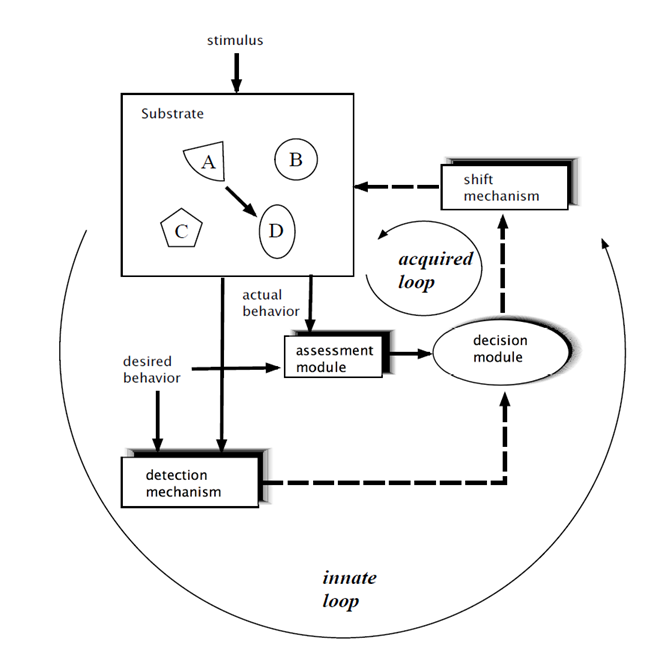
\includegraphics[scale=0.8]{ciclo_evolutivo.png}
\caption{Ciclo evolutivo di un sistema metamorfico}\label{fig:1}
\end{figure}

Il ciclo di vita di un Hardware Metamorfico può essere rappresentato come nella figura \ref{fig:1}: il superciclo che compone questo sistema, chiamato ``ciclo innato'', ha un sotto-ciclo di acquisizione di stimoli, chiamato ``ciclo di acquisizione'', che, tramite il sottostrato di algoritmi di esecuzione, cambia il funzionamento del sistema in base al ``comportamento attuale'' e il ``comportamento desiderato''; con questi dati, tramite un modulo di valutazione degli stimoli e un meccanismo di investigazione (per valutare il comportamento desiderato rispetto al comportamento attuale), viene generato dal modulo di ``decisione'' il risultato che fa modificare l'intero sistema. Il ciclo innato successivamente fa rieseguire questo procedimento, in modo da permettere, potenzialmente all'infinito, la metamorfosi del sistema.


\begin{thebibliography}{1}
\bibitem{MS1} Garrison W. Greenwood,Senior Member, IEEE and Andy M. Tyrrell,Senior Member, IEEE, ``\textit{Metamorphic Systems: A New Model for Adaptive System Design''}, 2010
\bibitem{EIE} Sekanina, L. ; Brno Univ. of Technol., Brno ; Martinek, T. ; Gajda, Z., \textit{Extrinsic and Intrinsic Evolution of Multifunctional Combinational Modules}, 2006
\end{thebibliography}

\end{document}
